%%%%%%%%%%%%%%%%%%%%%%%%%%%%%%%%%%%%%%%%%%%%%%%%%%%%%%%%%%%%%%%%%%%%%%%%%%%%%%%%
%%%%%%%%%%%%%%%%%%%%%%%%%%%%%%%%%%%%%%%%%%%%%%%%%%%%%%%%%%%%%%%%%%%%%%%%%%%%%%%%
%%                           AUTHOR: BIBEKANANDA DATTA                        %%
%%                               (C) MARCH 2024                               %%
%%                      PhD STUDENT, MECHANICAL ENGINEERING                   %%
%%                           JOHNS HOPKINS UNIVERSITY                         %%
%%%%%%%%%%%%%%%%%%%%%%%%%%%%%%%%%%%%%%%%%%%%%%%%%%%%%%%%%%%%%%%%%%%%%%%%%%%%%%%%
%%%%%%%%%%%%%%%%%%%%%%%%%%%%%%%%%%%%%%%%%%%%%%%%%%%%%%%%%%%%%%%%%%%%%%%%%%%%%%%%
%%             PLEASE CHECK THE README.md FILE BEFORE YOU PROCEED             %%
%%              it may be convenient to read this file on GitHub              %%
%%   GitHub: https://github.com/bibekananda-datta/JHU-Dissertation-Template   %%
%% template hosted on this GitHub repository is likely to be the most updated %%
%%%%%%%%%%%%%%%%%%%%%%%%%%%%%%%%%%%%%%%%%%%%%%%%%%%%%%%%%%%%%%%%%%%%%%%%%%%%%%%%

%%%%%%%%%%%%%%%%%%%%%%%%%%%%%%%%%%%%%%%%%%%%%%%%%%%%%%%%%%%%%%%%%%%%%%%%%%%%%%%%
% This is an unofficial dissertation template for Johns Hopkins University.
% As of March 31, 2024, the template follows the dissertation formatting 
% requirements provided by the  Johns Hopkins University Sheridan Library.
% It is the user's responsibility to ensure that the current requirements are 
% followed: https://www.library.jhu.edu/library-services/electronic-theses-dissertations/formatting-requirements/
%%%%%%%%%%%%%%%%%%%%%%%%%%%%%%%%%%%%%%%%%%%%%%%%%%%%%%%%%%%%%%%%%%%%%%%%%%%%%%%%
%%%%%%%%%%%%%%%%%%%%%%%%%%%%%% VERSION HISTORY %%%%%%%%%%%%%%%%%%%%%%%%%%%%%%%%%
% The report class-based template was created by R. Jacob Vogelstein in May 2007
% Updated by Noah J. Cowan on March 01, 2010
% Updated by Brian D. Weitzner on April 29, 2014 
% Updated by John Muschelli on January 29, 2016 
% Updated by Leonardo Collado Torres on April 13, 2016 
% Updated by John Clayton in December 2019
% Last Updated by Bibekananda Datta on March 31, 2024
%%%%%%%%%%%%%%%%%%%%%%%%%%%%%% VERSION HISTORY %%%%%%%%%%%%%%%%%%%%%%%%%%%%%%%%%


%%%% REPORT CLASS with 12 pt font and onesided printing (book class also works)
\documentclass[12pt,letterpaper]{report} 

%%%%%%%%%%%%%%%%%%%%%%%%%%%%%%%%%%%%%%%%%%%%%%%%%%%%%%%%%%%%%%%%%%%%%%%%%%%%%%%%
%% if possible, make your formatting changes here through the variables 
%%%%%%%%%%%%%%%%%%%%%% LIST OF VARIABLES FOR FORMATTING %%%%%%%%%%%%%%%%%%%%%%%%

%%%% JH Library requirement (DO NOT CHANGE)
\def\GlobalMargin{1.0in}                    % margin on all sides
\def\PrintingOffset{0.5in}                  % additional left margin for the printed copy
\def\MainTextSpacing{\doublespacing}        % double-spaced main text


%%%% ADDITIONAL PATHS and FILES
\def\FigurePath{figures}                    % subdirectory for the figure files
\def\BibFileName{thesis.bib}                % name of BibLaTeX-compatible bib file 


\def\FontPackage{lmodern}                   % default font package


%%%% FONT SIZE and TYPESET for DIFFERENT HEADINGS
%% check here for details: https://en.wikibooks.org/wiki/LaTeX/Fonts

%% font format for thesis title
\def\TitleFont{\Large\bfseries\singlespacing\MakeUppercase}  

%% font for chapter, section, subsection, and subsubsection heading
\def\NoSectionLevel{3}                      % 3 levels => section to subsubsection
\def\ChapterFont{\Large\bfseries\singlespacing} 
\def\SectionFont{\large\bfseries\singlespacing} 
\def\SubsectionFont{\normalsize\bfseries\singlespacing}  
\def\SubsubsectionFont{\normalsize\itshape\singlespacing} 


%%%% PARAGRAPH
\def\ParagraphSpacing{\baselineskip}        % spacing between paragraph
\def\ParagraphIndent{0 pt}                  % indentation at the beginning of the paragraph


%% CAPTION
\def\CaptionFontSize{small}         % caption font size
\def\CaptionLabelFontType{bf}       % boldface label for captions
\def\CaptionSeparator{colon}        % separates caption label from caption text
\def\CaptionSpacing{1.0}            % single-spaced captions
\def\FigureToCaption{0 pt}          % spacing between the figure and the caption


%%%% GLOBAL SPACING for TABLES
\def\GlobalTableSpacing{1.5}                % global spacing parameter for table


%%%% HEADER AND FOOTER SETTING
\def\HeaderHeight{30 pt}                    % height of the chapter header
\def\HeaderSpace{12 pt}                     % space between header and the following text

\def\FootnoteSpacing{\baselineskip}         % spacing between footnotes


%%%% BIBLIOGRAPHY ITEMS
\def\BibTextSpacing{\singlespacing}         % single-spaced bibliography
\def\BibItemSpacing{\baselineskip}          % spacing between bibliographic items in reference


%%%% CHAPTER QUOTE (EPIGRAPH PACKAGE)
\def\ChapQuoteFontSize{\small}              % font size of chapter quotes
\def\ChapQuoteLocation{flushright}          % location of chapter quote
\def\ChapQuoteTextShape{\itshape}           % font shape for quotes
\def\ChapQuoteAuthorTextShape{\scshape}     % font shape for quote author
\def\MaxQuoteWidth{0.65\textwidth}          % width epigraph-based quotes in chapter



%%%% SECTION LEVELS and TOC APPEARANCE
\def\NoTocLevel{2}                          % no of levels showed in the table of contents
\def\TocIndent{0 pt}                        % indentation in the list of figs and tables
%% 3 levels mean: section to subsubsection.. decrease if you want to show less in TOC

%%%% TOC SPACING of different section levels (chapter to subsubsection)
\def\TOCTextSpacing{\singlespacing}         % single spacing for TOC texts
\def\ChapTOCSpacing{\baselineskip}          % spacing between chapters
\def\SecTOCSpacing{0.5\baselineskip}        % spacing between sections
\def\SubsecTOCSpacing{0.3\baselineskip}     % ... between subsections
\def\SubsubsecTOCSpacing{0.3\baselineskip}  % ... between subsubsections
\def\LOTItemSpacing{\baselineskip}          % spacing between LOT/LOF items


%%%% ADHOC HEIGHT ADJUSTMENT VARIABLES for consistent typesettings
%% following numbers are found by trial and error to compensate 
%% for default spacing around default LaTeX environments
\def\TitleTopSpacing{-\HeaderHeight-\HeaderSpace}   % top height adjustment for thesis title
\def\BeforeTOCTitleSpacing{-42 pt}          % space before TOC title
\def\AfterTOCTitleSpacing{34 pt}            % space after TOC title
\def\AfterLOTTitleSpacing{34 pt}            % space after LOT/ LOF title

\def\NumChapterTopMargin{-64 pt}            % space before numbered chapter label
\def\UnNumChapterTopMargin{-85 pt}          % space before unnumbered chapter label
\def\ChapLabelToTitle{-27 pt}               % space between chapter label to title 
\def\ChapTitleToText{24 pt}                 % space between the chapter title and the following text
\def\SpaceBeforeQuote{-20 pt}               % white space before quote

%%%% if you want to change any of the heights, adjust using a ruler:
% \usepackage[unit=in,type=upperleftT,color=red,showframe]{fgruler}

%%%%%%%%%%%%%%%%%%%% END LIST OF VARIABLES FOR FORMATTING %%%%%%%%%%%%%%%%%%%%%%


%%%%%%%%%%%%%%%%%%%%%%%%%%%%%%%%%%%%%%%%%%%%%%%%%%%%%%%%%%%%%%%%%%%%%%%%%%%%%%%%
%% add packages as needed but sometimes the order of the packages matters.
%% you may have to change the options of the biblatex package for the bibliography.
%%%%%%%%%%%%%%%%%%%%%%%%%%%%%%% LaTeX PACKAGES %%%%%%%%%%%%%%%%%%%%%%%%%%%%%%%%%

%%%% SOME PRE-REQUISITE PACKAGES
\usepackage[utf8]{inputenc}                 % for encoding input character (required)
\usepackage[american]{babel}                % for different language typography
\usepackage[T1]{fontenc}                    % for font encoding


%%%% COMMON MATH PACKAGES
\usepackage{amsfonts,amssymb,amsmath,amsthm,autobreak,
cancel,dsfont,mathtools,mathbbol,mathrsfs,siunitx,upgreek}


%%%% DEFAULT FONT (you can specify other fonts - compatibility could be an issue)
\usepackage{\FontPackage}


%%%% BIBLIOGRAPHIC PACKAGE (change the style or other options if you need to)
%% Nature style bibliography
\usepackage[backend=biber, defernumbers=true, style=nature, maxnames=99,
     date=year, isbn=false, url=false, doi=true]{biblatex}

%% APA style
% \usepackage[backend=biber, defernumbers=true, style=apa, maxnames=99,
%     isbn=false, url=false, doi=true]{biblatex}

%% IEEE style
% \usepackage[backend=biber,style=ieee,defernumbers=true,maxnames=99, 
%     date=year, isbn=false, url=false, doi=true]{biblatex}



%%%% TABLE-RELATED PACKAGES
\usepackage{booktabs,longtable,dcolumn,makecell,
multicol,multirow,tabularx,xltabular,rotating}



%%%% package for micro-typography (you can define more settings)
%% see details here: https://www.khirevich.com/latex/microtype/
\usepackage[activate={true,nocompatibility}]{microtype}



%%%% OTHER PACKAGES AND OPTIONS
\usepackage[pagewise,mathlines]{lineno}     % line numbers for drafting
\usepackage[ruled]{algorithm2e}             % to manage algorithm environment
\usepackage[titletoc]{appendix}             % to manage appendix chapters
\usepackage{blindtext}                      % to generate random filler texts
\usepackage{calc}                           % to set arithmetic arguments for spacing
\usepackage{caption}                        % to manage captions
\usepackage{comment}                        % to comment a large amount of text as env
\usepackage{epigraph,varwidth}              % for managing quotes
\usepackage{enumitem}                       % to manage list environment
\usepackage{float}                          % to manage floating environment
% footnote environment management
\usepackage[bottom,multiple,hang,flushmargin]{footmisc}      
\usepackage{graphicx,wrapfig}               % to manage images
\usepackage{geometry}                       % to manage margins and page format
\usepackage{glossaries}                     % to add glossaries
\usepackage{fancyhdr}                       % for header/ footer settings
\usepackage[dvipsnames]{xcolor}             % color-related package
\usepackage[a-1b]{pdfx}                     % to generate PDF/A file (before hyperref)
\usepackage[pdfa]{hyperref}                 % for hyperlink management 
\usepackage[all]{hypcap}                    % for captions on the side of figures
\usepackage{ifthen}                         % if-then statement in LaTeX code
\usepackage{lscape}                         % landscape mode
\usepackage{listings,minted}                % to include codes 
\usepackage{csquotes}                       % yet another package to manage quote
\usepackage{setspace}                       % sets space between lines
\usepackage{seqsplit}                       % splits long character sequence
\usepackage[rightcaption]{sidecap}          % for sideway captions
\usepackage{tocloft}                        % to manage table of contents, etc.
\usepackage{textcomp}                       % text companion fonts in TS1
\usepackage[absolute]{textpos}              % position text at certain location
\usepackage{titlesec}                       % managing different title environments
\usepackage[final]{pdfpages}                % to insert pdf pages
\usepackage{parskip}                        % default spacing around environments
\usepackage{tikz}                           % drawing related package
\usepackage{subcaption}                     % individual panel and caption

%% add more packages and/or change options of the packages as needed

%%%%%%%%%%%%%%%%%%%%%%%%%%%%%% END LaTeX PACKAGES %%%%%%%%%%%%%%%%%%%%%%%%%%%%%



%%%%%%%%%%%%%%%%%%%%%%%%%%%%%%%%%%%%%%%%%%%%%%%%%%%%%%%%%%%%%%%%%%%%%%%%%%%%%%%
%% specifying direct package options related to document formatting
%%%%%%%%%%%%%%%%%%%%%%%%%%%%%% PACKAGE OPTIONS %%%%%%%%%%%%%%%%%%%%%%%%%%%%%%%%

%%%% GRAPHICX package
\graphicspath{{\FigurePath/}}


%%%% GEOMETRY PACKAGE: margin settings required by JH library 
\geometry{letterpaper, margin=\GlobalMargin, bindingoffset=\PrintingOffset, 
    nomarginpar, includehead, headheight=\HeaderHeight, 
    headsep=\HeaderSpace, includefoot, heightrounded}
%% you can add showframe option to see how the layout looks like


%%%% HYPERREF PACKAGE
\hypersetup{linktocpage, unicode, linktoc=all, colorlinks=true, 
    citecolor=blue, filecolor=blue, linkcolor=blue, urlcolor=blue}
\urlstyle{rm}           % removes default \texttt style for hyperlinks


%%%% CAPTION PACKAGE
\captionsetup{belowskip=\FigureToCaption, font=\CaptionFontSize, 
    labelfont=\CaptionLabelFontType, labelsep=\CaptionSeparator,
    font={stretch=\CaptionSpacing}, hypcap=true} 



%%%% BIBLATEX: bibliography package settings
\addbibresource{\BibFileName}           % name of the bib file 
% \DeclareFieldFormat{titlecase}{\MakeSentenceCase*{#1}}
\AtBeginBibliography{\urlstyle{rm}}     % roman font family for URL (DOI)
\AtBeginBibliography{\vspace*{8pt}}     % add space for single-spaced bib text

%% the following block ensures articles are sentence case 
%% but the journal names are title case 
\DeclareFieldFormat{sentencecase}{\MakeSentenceCase{#1}}
\renewbibmacro*{title}{%
  \ifthenelse{\iffieldundef{title}\AND\iffieldundef{subtitle}}
    {}
    {\ifthenelse{\ifentrytype{article}\OR\ifentrytype{inbook}%
      \OR\ifentrytype{incollection}\OR\ifentrytype{inproceedings}%
      \OR\ifentrytype{inreference}}
      {\printtext[title]{%
        \printfield[sentencecase]{title}%
        \setunit{\subtitlepunct}%
        \printfield[sentencecase]{subtitle}}}%
      {\printtext[title]{%
        \printfield[titlecase]{title}%
        \setunit{\subtitlepunct}%
        \printfield[titlecase]{subtitle}}}%
     \newunit}%
  \printfield{titleaddon}}


%% separate category for papers to be not cited in the bibliography
\DeclareBibliographyCategory{mypapers}             
\newcommand{\mybibexclude}[1]{\addtocategory{mypapers}{#1}}

%%%%%%%%%%%%%%%%%%%%%%%%%%%% END PACKAGE OPTIONS %%%%%%%%%%%%%%%%%%%%%%%%%%%%%%%


%%%%%%%%%%%%%%%%%%%%%%%%%%%%%%%%%%%%%%%%%%%%%%%%%%%%%%%%%%%%%%%%%%%%%%%%%%%%%%%
%% further tweaking variables for the current consistent document formatting
%%%%%%%%%%%%%%%%%%%%%%%%%%%%% DOCUMENT FORMATTING %%%%%%%%%%%%%%%%%%%%%%%%%%%%%%

\setcounter{tocdepth}{\NoTocLevel}                  % list depth in ToC
\setcounter{secnumdepth}{\NoSectionLevel}           % section to ... subsubsection


%%%% font size and spacing around the titles of ToC/ LoT/ LoF
\renewcommand{\cfttoctitlefont}{\ChapterFont}
\renewcommand{\cftlottitlefont}{\ChapterFont}
\renewcommand{\cftloftitlefont}{\ChapterFont}

\setlength{\cftbeforetoctitleskip}{\BeforeTOCTitleSpacing}
\setlength{\cftbeforelottitleskip}{\BeforeTOCTitleSpacing}
\setlength{\cftbeforeloftitleskip}{\BeforeTOCTitleSpacing}
\setlength{\cftaftertoctitleskip}{\AfterTOCTitleSpacing}
\setlength{\cftafterlottitleskip}{\AfterLOTTitleSpacing}
\setlength{\cftafterloftitleskip}{\AfterLOTTitleSpacing}


%% tweak to TOC to add 'chapter' to the chapter name instead of a number only
%% set the width of the box based on the longest label name
\renewcommand{\cftchappresnum}{\chaptername\space}
\renewcommand{\cftchapleader}{\cftdotfill{\cftdotsep}}  % dots for chapters too
\setlength{\cftchapnumwidth}{\widthof{\textbf{Appendix~XXX~}}}


\setlength{\cftbeforechapskip}{\ChapTOCSpacing}
\setlength{\cftbeforesecskip}{\SecTOCSpacing}
\setlength{\cftbeforesubsecskip}{\SubsecTOCSpacing}
\setlength{\cftbeforesubsubsecskip}{\SubsubsecTOCSpacing}


%% tweak to LOT and LOF to add 'Table'/ 'Figure' to the table/ figure caption listing
%% to change the distance to the start of the table/ figure title
\newcommand*{\noaddvspace}{\renewcommand*{\addvspace}[1]{}}

\setlength{\cfttabindent}{\TocIndent}               % indentation from tables in LoT
\renewcommand{\cfttabpresnum}{\bfseries Table }
\setlength{\cfttabnumwidth}{\widthof{\textbf{Table~999.999~}}}
\setlength{\cftbeforetabskip}{\LOTItemSpacing}      % spacing between each item
\addtocontents{lot}{\protect\noaddvspace}


\setlength{\cftfigindent}{\TocIndent}               % indentation from figures in LoF
\renewcommand{\cftfigpresnum}{\bfseries Figure }
\setlength{\cftfignumwidth}{\widthof{\textbf{Figure~999.999~}}}
\setlength{\cftbeforefigskip}{\LOTItemSpacing}      % spacing between each item
\addtocontents{lof}{\protect\noaddvspace}



%%%% TITLESEC: settings for chapter label and title
\titleformat{\chapter}[display]{\ChapterFont}
    {\chaptertitlename\ \thechapter}{\ChapLabelToTitle}{\ChapterFont}

\titlespacing*{\chapter}{0pt}{\NumChapterTopMargin}{\ChapTitleToText} 

\titlespacing*{name=\chapter,numberless}{0pt}{\UnNumChapterTopMargin}
    {\ChapTitleToText}


%%%% TITLESEC: settings for sections, subsection, ... heading format
\titleformat*{\section}{\SectionFont}
\titleformat*{\subsection}{\SubsectionFont}
\titleformat*{\subsubsection}{\SubsubsectionFont}
%% if you had more levels then add settings for paragraph and subparagraph


%% to customize space around section headings, use the following command:
% \titlespacing*{environment-name}{space-left}{space-before}{space-after}


%%%% PARSKIP: for paragraph (and not title) spacing, roughly speaking
\renewcommand{\arraystretch}{\GlobalTableSpacing}   % spacing inside table
\setlength{\parskip}{\ParagraphSpacing}             % paragraph skip
\setlength{\parindent}{\ParagraphIndent}            % paragraph indentation
\setlength{\bibitemsep}{\BibItemSpacing}            % bib item separation 
\setlength{\footnotesep}{\FootnoteSpacing}          % separation between footnote


%%%% settings for math environment
\allowdisplaybreaks[1]                  % page break for long equations
\numberwithin{equation}{chapter}        % eqn no with chapter label
\setcounter{MaxMatrixCols}{20}          % no of maximum columns in matrix

%%%%%%%%%%%%%%%%%%%%%%%%%%% END DOCUMENT FORMATTING %%%%%%%%%%%%%%%%%%%%%%%%%%%

%%%%%%%%%%%%%%%%%%%%%%%%%%%%% TITLE PAGE MACROS %%%%%%%%%%%%%%%%%%%%%%%%%%%%%%%

\newcommand{\ThesisTitle}[1]{           % thesis title
    \vspace*{\TitleTopSpacing}
    {\TitleFont {#1} \par}
}

\newcommand{\ThesisAuthor}[1]{          % thesis author
    by \\ #1 \\}      


\newcommand{\ThesisStatement}[2]{       %% thesis or dissertation statement 
    A {#1} submitted to The Johns Hopkins University in conformity \\
    with the requirements for the degree of {#2}
}

\newcommand{\Location}{Baltimore, Maryland}     % location

\newcommand{\ThesisDate}[2]{#1 #2}              % thesis submission date 

\newcommand{\ThesisCopyright}[2]{               % optional copyright statement
\begin{textblock*}{\textwidth}(\GlobalMargin +\PrintingOffset,9in)
    \copyright\ {#1} {#2} \\ All rights reserved
\end{textblock*}
\null
}

%%%%%%%%%%%%%%%%%%%%%%%%%%% END TITLE PAGE MACROS %%%%%%%%%%%%%%%%%%%%%%%%%%%%%


%%%%%%%%%%%%%%%%%%%%%%%%%%%%%% OTHER MACROS %%%%%%%%%%%%%%%%%%%%%%%%%%%%%%%%%%%

%%%% UNNUMBERED CHAPTERS, SECTION, and SUBSECTION COMMAND for ADDING to TOC
%% removes the 'Chapter #' title while keeping it listed in the TOC
\newcommand\chap[1]{%
    \chapter*{#1}%
    \markboth{#1}{}
    \addcontentsline{toc}{chapter}{#1}}
  
%% removes the 'Section #' title while keeping it listed in the TOC
\newcommand\sect[1]{%
    \phantomsection
    \section*{#1}%
    \addcontentsline{toc}{section}{#1}}
  
%% removes the 'Subsection #' title while keeping it listed in the TOC
\newcommand\subsect[1]{%
    \phantomsection
    \subsection*{#1}%
    \addcontentsline{toc}{subsection}{#1}}

%% removes the 'Subsubsection #' title while keeping it listed in the TOC
\newcommand\subsubsect[1]{%
    \phantomsection
    \subsubsection*{#1}%
    \addcontentsline{toc}{subsubsection}{#1}}

%%%% KEYWORDS for abstract
\newcommand{\keywords}[1]{	
    \textbf{Keywords:} {#1}
}

%%%% TOCLOFT: modified macros/ commands for printing ToC, LoF, LoT
\newcommand{\mytableofcontents}{
    \clearpage
    \renewcommand{\contentsname}{Table of Contents}
    \tableofcontents
    \clearpage
}
%
\newcommand{\mylistoffigures}{
    \clearpage \phantomsection
    \addcontentsline{toc}{chapter}{List of Figures}
    \listoffigures
    \clearpage
}
%
\newcommand{\mylistoftables}{
    \clearpage \phantomsection
    \addcontentsline{toc}{chapter}{List of Tables}
    \listoftables
    \clearpage
}

%%%% IN-TEXT MACROS for notes
\newcommand{\COMMENT}{\textcolor{red}}
\newcommand{\ADDCITATION}{\COMMENT{(ADD CITATION)}}

%%%%%%%%%%%%%%%%%%%%%%%%%%%% END OTHER MACROS %%%%%%%%%%%%%%%%%%%%%%%%%%%%%%%%%



%%%%%%%%%%%%%%%%%%%%%%%%%%%%%%%%%%%%%%%%%%%%%%%%%%%%%%%%%%%%%%%%%%%%%%%%%%%%%%%
%% only if you plan on using chapter quotes, you may need epigraph settings
%%%%%%%%%%%%%%%%%%%%%%%%%%%%% EPIGRAPH SETTINGS %%%%%%%%%%%%%%%%%%%%%%%%%%%%%%%

\setlength{\epigraphwidth}{\MaxQuoteWidth}              % max width of chapter epigraph
\renewcommand{\epigraphflush}{\ChapQuoteLocation}       % chapter epigraph on right 
\renewcommand{\epigraphsize}{\ChapQuoteFontSize}        % font size for chapter epigraph
\renewcommand{\textflush}{\ChapQuoteLocation}
\renewcommand{\sourceflush}{\ChapQuoteLocation}
\newcommand{\epitextfont}{\ChapQuoteTextShape}          % quote font shape
\newcommand{\episourcefont}{\ChapQuoteAuthorTextShape}  % quote author name shape

%% following settings put variable width underline between quote and author
\makeatletter
\setlength{\beforeepigraphskip}{\SpaceBeforeQuote}
\newsavebox{\epi@textbox}
\newsavebox{\epi@sourcebox}
\newlength\epi@finalwidth
\renewcommand{\epigraph}[2]{%
    \vspace{\beforeepigraphskip}
    {\epigraphsize\begin{\epigraphflush}
    \epi@finalwidth=\z@
    \sbox\epi@textbox{%
        \varwidth{\epigraphwidth}
        \begin{\textflush}\epitextfont#1\end{\textflush}
        \endvarwidth
   }%
    \epi@finalwidth=\wd\epi@textbox
    \sbox\epi@sourcebox{%
        \varwidth{\epigraphwidth}
        \begin{\sourceflush}\episourcefont#2\end{\sourceflush}%
        \endvarwidth
   }%
    \ifdim\wd\epi@sourcebox>\epi@finalwidth 
        \epi@finalwidth=\wd\epi@sourcebox
    \fi
   \leavevmode\vbox{
        \hb@xt@\epi@finalwidth{\hfil\box\epi@textbox}
        \vskip 1ex         % gap between quote and rule
        \hrule height \epigraphrule
        \vskip 1ex         % gap between rule and author
        \hb@xt@\epi@finalwidth{\hfil\box\epi@sourcebox}
   }%
   \end{\epigraphflush}
   \vspace{\afterepigraphskip}}}
\makeatother

%%%%%%%%%%%%%%%%%%%%%%%%%%% END EPIGRAPH SETTINGS %%%%%%%%%%%%%%%%%%%%%%%%%%%%%

%%% define your custom settings for other packages here (algorithm/ listing, etc.)


%%%%%%%%%%%%%%%%%%%%%%%%%%%%%%%%%%%%%%%%%%%%%%%%%%%%%%%%%%%%%%%%%%%%%%%%%%%%%%%
%% these are just some examples; add more macros for your custom commands
%%%%%%%%%%%%%%%%%%%%%%%%%%%%%% MATH MACROS %%%%%%%%%%%%%%%%%%%%%%%%%%%%%%%%%%%%

\newcommand{\dC}{$^{\circ}$C}           % degree celsius symbol
\newcommand{\vect}[1]{\mathbf{#1}}      % boldface for vectors and tensors
\DeclareMathOperator{\T}{{\top}}        % transpose of a matrix/ tensor
\DeclareMathOperator{\tr}{tr}           % trace of a matrix
\DeclareMathOperator{\divg}{div}        % divergence of vector and tensor
\DeclareMathOperator{\grad}{grad}       % gradient of vector and tensor
\DeclareMathOperator{\curl}{curl}       % curl of vector and tensor

%% theorem-style remark environment
\theoremstyle{definition}
\newtheorem{remark}{Remark}

%%%%%%%%%%%%%%%%%%%%%%%%%%%%% END MATH MACROS %%%%%%%%%%%%%%%%%%%%%%%%%%%%%%%%%



%%%%%%%%%%%%%%%%%%%%%%%%% DOCUMENT BEGINS HERE %%%%%%%%%%%%%%%%%%%%%%%%%%%


\begin{document}


%%%% TITLE PAGE
%%%% JHU Dissertation title page (if you are not sure, do not change the formatting)

\begin{titlepage}

% centered single-spaced title page w/ no page numbering
\begin{center}
\singlespacing  \thispagestyle{empty}       

%%%% thesis title: 1.5 inches from the top of the page
\ThesisTitle{\LaTeX\ Dissertation Template for Johns Hopkins University}

\vspace{1in}                    % gap between the title and the author: approx. 1 inch

\ThesisAuthor{John Doe}         % author name for the thesis

\vspace{1.5in}                  % gap between the author and statement: 1.5 inches

%%%% for masters change arguments to: {thesis}{masters program name}
\ThesisStatement{dissertation}{Doctor of Philosophy}  
%% gap between statement and location: approx. 0.5 inch
\vspace{0.5in} \\               

\Location \\                    % prints Baltimore, Maryland as the location
\ThesisDate{Month}{YEAR}        % thesis submission month and year (single-spaced)


%%%% optional copyright statement: approx. 2 inches from the bottom of the page
%% year and name are input argument for copyright statement
\ThesisCopyright{YEAR}{John Doe}


\end{center}

\end{titlepage}
        

%%%%%%%%%%%%%%%%%%%%%%%%%%%% FRONT MATTER %%%%%%%%%%%%%%%%%%%%%%%%%%%%%%%%

%%%% text spacing, page numbering, and header settings
\MainTextSpacing                            % double spacing for the contents
\pagenumbering{roman}                       % pagination style: Roman numeral
\setcounter{page}{2}                        % page counter starts at roman ii
\pagestyle{fancy}
\renewcommand{\chaptermark}[1]{\markboth{#1}{#1}}
\fancyhead[R]{}               
\fancyhead[L]{\nouppercase \leftmark}       % prints header for unnumbered chap


%%%% MUST ADD ABSTRACT (includes committee as well)
\chap{Abstract} 

%% your abstract goes here (add your abstract)
\Blindtext[3]


%%%%  committee members go here (do not go to a new page; 
%%% it should be right after the abstract)
\begin{singlespace}

\subsection*{Primary reader and thesis advisor:}

Dr. Chuck Darwin \\
Professor\\
Department of Biology\\
Johns Hopkins University, Baltimore MD 

\vspace{0.25in}

\subsection*{Secondary readers: }

Dr. Stewart Hawking\\
Professor\\
Department of Biology \\
Johns Hopkins University, Baltimore, MD 

\vspace{0.1in}

Dr.~Jimmy Watson \\
Professor\\
Department of Biology \\
Johns Hopkins University, Baltimore, MD 

%%%% add more readers if you have in your committee 
%%%% using \vspace{0.1in} in between them

\end{singlespace}


%%%% OPTIONAL but COMMON: preface chapters
\chapter*{~}
\addcontentsline{toc}{chapter}{Dedication}
%% did not use \chap command because the chapter does not have any name

%%%% there is no format for this page. depending on your text, 
%%%% you can adjust the height and style of the text
\begin{center}
\vspace*{2.5in}
    \textit{This thesis is dedicated to ...}
\end{center}

\chap{Acknowledgement}

%%%% there is no specific formatting requirement for this section 
%% default is double-spaced (you can style it as you want)
TODO

Ram Kripa: help with coding and deployment 

Amanda Ferber: help with scraping and database creation

Prof David yarowsky 

Prof Joshua Reiter         
%\chapter*{~}
%\addcontentsline{toc}{chapter}{Epigraph}

%% it is a less common optional page with no specific requirement

%\begin{center}                      % horizontal centering of the texts
%\vspace*{2.5in}                     % adjust the space to place vertically centered
%\begin{onehalfspacing}
%    \textit{
%    Veritas vos liberabit \\
    %The truth will set you free 
%    } \\
    
    %\rule{1.5in}{0.5pt} \\          % legth and thickness of the rule
    
    %\textsc{John 8:32}
%\end{onehalfspacing}
%\end{center}
%% you can have other chapters and the order does not matter



%%%% LISTINGS
\microtypesetup{protrusion=false}
\TOCTextSpacing                             % one-half spacing for the table of contents
\hypersetup{linkcolor=black}                % local black hyperlink for TOC
%
\mytableofcontents                          % MUST
%
\mylistoftables                             % MUST: if you have tables
%
\mylistoffigures                            % MUST: if you have figures
%
%% OPTIONAL: you can add more lists here (but you will have to define those)
%
\microtypesetup{protrusion=true}

%%%%%%%%%%%%%%%%%%%%%%%%%%% END FRONT MATTER %%%%%%%%%%%%%%%%%%%%%%%%%%%%


%%%%%%%%%%%%%%%%%%%%%%%%%%%%% MAIN MATTER %%%%%%%%%%%%%%%%%%%%%%%%%%%%%%%

%%%% PAGE and TEXT settings 
\MainTextSpacing                        % restores double spacing 
\pagenumbering{arabic}                  % Arabic page numbering
\fancyhead[L]{\chaptername\ \thechapter. \nouppercase \leftmark}


%%%% include all the main text chapters
\chapter{Chapter title goes here} \label{chap:chap-1}

% if you want a short header you can use the following command
% \chapter[short-header-name]{chapter-title} \label{chap:chap-1}


%% add your chapter text here
\blindtext \cite{dirac}

\Blindtext[3]


\chapter{Literature Review} \label{chap:chap-2}

%%%% OPTIONAL EPIGRAPH EXAMPLE
%\epigraph{Do not believe everything you see on the internet.}{-- Albert Einstein}


%%%% MUST: if the chapter is a reprint or submitted paper, you must declare it
%% you can use enumerate or itemize environment if you have more than one paper 
%% \mybibexclude{} will exclude this citation from the final bibliography
%% if this paper appears somewhere else then remove \mybibexclude{} command

%\begin{singlespace}         % you can also use `onehalfspace` to relax the spacing
%    This chapter is adapted from the following article with permission from <publisher>
    
%    \fullcite{einstein}. \mybibexclude{einstein}
%\end{singlespace} 


%%%% remove the following and add your chapter text here
\section{Introduction}
The growing demand for technical skills has led many learners to open-access courseware platforms like Coursera and edX. While these platforms offer a wealth of quality educational content, they also present challenges, such as navigating a vast selection of courses, identifying those that align with individual goals, and understanding prerequisite requirements. 

This leads to choice overload, where too many options and insufficient guidance result in frustration and poor learning outcomes. Existing recommendation systems rely on vanilla algorithms that prioritize popular courses or basic keyword matching, and fail to capture the unique needs and diverse backgrounds of learners. Recent advancements in AI, particularly through Large Language Models (LLMs) and Retrieval-Augmented Generation (RAG), offer new opportunities to address these challenges. By providing more dynamic and context-aware recommendations, these models can create personalized experiences. 

This chapter explores the obstacles faced by self-learners, the limitations of existing recommendation systems, and how LLMs can reshape personalized learning. It also identifies the key features of an effective system and the remaining gaps in current solutions.

\section{AI is Changing Every Field} 

Advancements in Artificial Intelligence (AI) are transforming a wide range of industries \cite{nature:2023} and driving the demand for technical skills and Computer Science knowledge \cite{tamayo:2023}. From healthcare \cite{saxena:2024} to education \cite{luckin:2016} and creative industries \cite{almamari:2024}, AI is enabling new innovations that require expertise in areas such as Data Science, Machine Learning, and Software Development. In sectors like healthcare, AI is being used to analyze large datasets, improve diagnostic accuracy \cite{lenharo:2023}, and enhance patient care \cite{ranjbar:2024}. Similarly, in finance, AI-powered algorithms are automating fraud detection and risk assessment \cite{shabir:2024}. These developments demonstrate the expanding influence of AI and highlight the increasing need for professionals with a strong technical foundation.

\subsection{There is a growing demand for technical skills}

As AI and technology continues to shape various fields, the demand for individuals with Computer Science knowledge has surged. According to recent studies, job postings requiring computer science and AI-related skills have increased significantly, emphasizing the rising value of these competencies in the job market \cite{bls:2024} \cite{wef:2020}. 

More professionals and learners are recognizing the value of technical expertise, both to remain competitive in their current roles and to explore new career paths \cite{abe:2020}. Moreover, a growing number of students and early-career professionals are seeking knowledge in these areas \cite{anderson:2023}. This influx of learners from diverse backgrounds creates new challenges in identifying educational resources that are both relevant and appropriate for their various needs.

\subsection{Traditional education is not enough }
However, traditional educational programs are often not well-suited to meet this growing demand \cite{shell:2018}. While university degrees offer comprehensive coursework, they are typically expensive and inflexible, making them inaccessible to many learners. These programs also struggle to meet the needs of continuing learners—those already in the workforce who wish to update their skills \cite{laal:2012}. High tuition costs and rigid schedules limit access to these traditional pathways, leaving many learners seeking alternative ways to gain the necessary expertise \cite{vargas:2023}.

\subsection{MOOCs}
For these reasons, an increasing number of learners are turning to more flexible and affordable options, such as open-access courseware and Massive Open Online Courses (MOOCs) \cite{harish:2013} \cite{papmpouri:2021}. The rise of Massive Open Online Courses marked a significant shift in the accessibility of education. MOOCs were initially celebrated for their potential to democratize education, offering a plethora of high-quality courses from leading universities to anyone with internet connection. 

In 2009, a meta-analysis by the U.S. Department of Education examined evidence-based practices in online learning and found that students in online learning conditions performed better on average than students receiving in-person instruction \cite{means:2009}. However, as the popularity of these platforms grew, studies revealed patterns of enrollment and attrition that highlighted several challenges. A preliminary case study on Australian open-access online education found that while MOOCs attracted a large and diverse group of enrollees, many learners struggled to stay engaged \cite{greenland:2014}. High attrition rates and low completion rates became characteristic of MOOCs, both emphasizing their capability for increasing access to education and raising concerns about their effectiveness in achieving long-term learning outcomes \cite{clow:2013}. 

\section{What a system/solution should include}

Synthesize everything 
- personalized and goal oriented
- take backgrounds into consideration + prerequisite stuff 

\chapter{Gaita Overview} \label{chap:chap-3}


% epigraph after chapter heading
\epigraph{Since it is written in \LaTeX, it must be true.}{-- Isaac Newton}


%%%% MUST: add the citation for the chapter if it is a reprint



%% remove the following and add your chapter text here
\section{Overview of Design and Purpose}
%\blindtext 

\subsection{Goals and Objectives}

\subsection{How users interact with Gaita to generate recommendations}

how input (background and goals) influence learning paths 

\section{Justification for Components} 
Justify components chosen; why and why not (reviews, these 2 sites) 

%\blindtext\footnote{Hello, this is the first footnote with no indentation and single-spaced text. The spacing between two footnotes is also single-spaced.}

\section{Data Sources}
\chapter{System Design and Architecture} \label{chap:chap-4}


\section{Architecture Diagram and Flow}

Gaita's architecture diagram outlines the flow of data and how various components work together to generate personalized learning pathways for users. Here is a breakdown of the system:

\begin{figure}[ht]
\begin{center}
    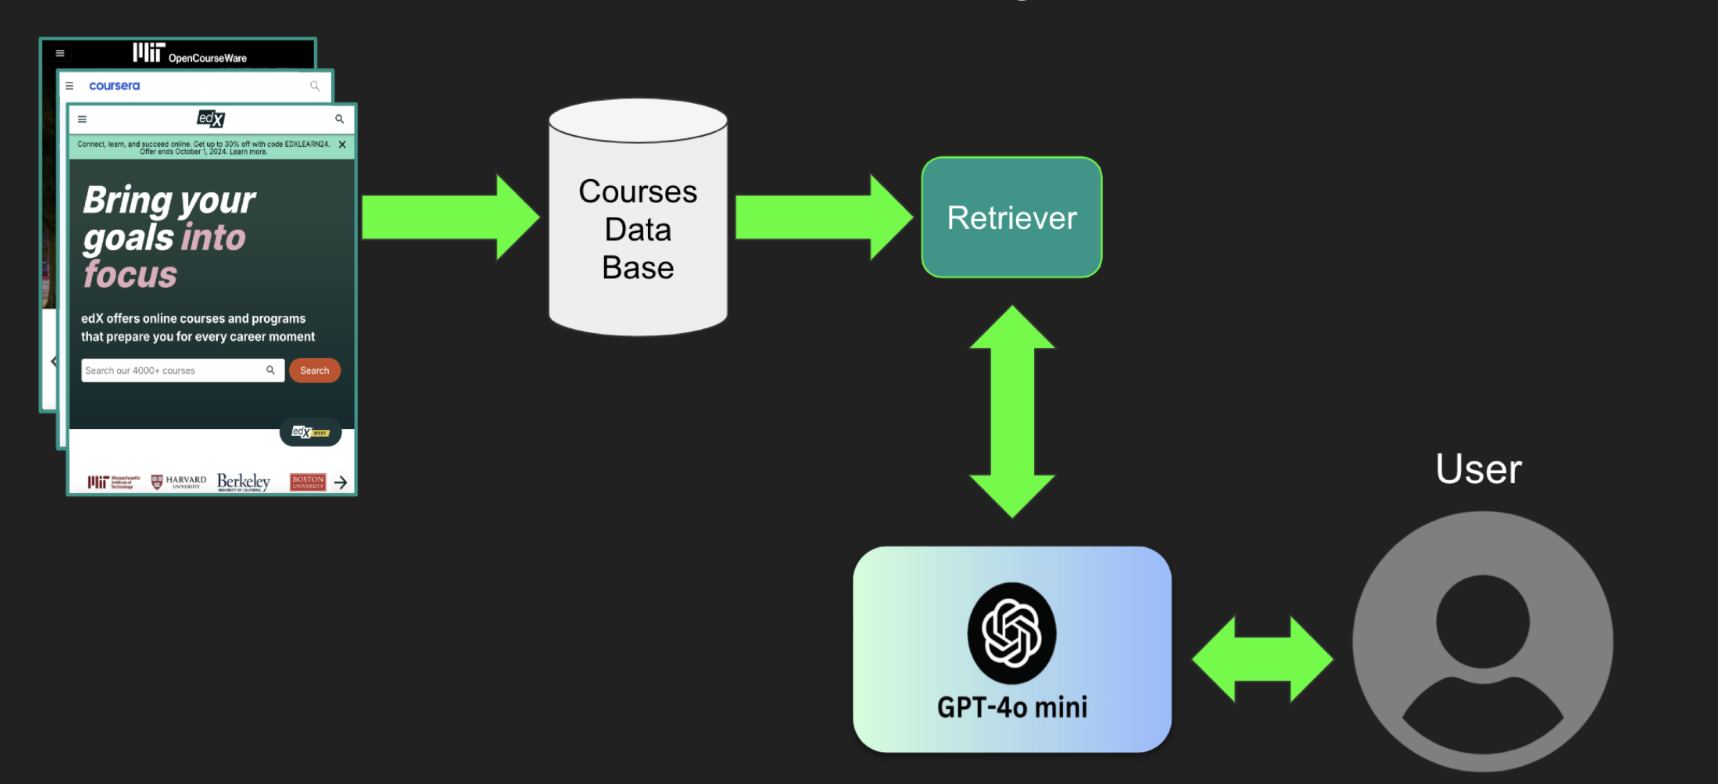
\includegraphics[width=\textwidth] {architecture_diagram.png}
    \caption{Gaita Architecture Diagram}
    \label{fig:architecture_diagram}
\end{center}
\end{figure}

\begin{enumerate}
\item \textbf{Scrape CS Courses from Coursera and MIT OCW:} Gaita collects course data from Coursera and MIT OpenCourseWare. These platforms provide high-quality Computer Science courses from leading institutions, ensuring a reliable and diverse range of learning materials.  

\item \textbf{Courses Database:} The courses from these platforms are scraped and stored in a central database. This database contains the titles, descriptions, and URLs of over 1,200 courses.

\item \textbf{Retriever:} The "Retriever" component is responsible for retrieving the most relevant courses based on the user’s input. Using cosine similarity, the system compares the vectorized user prompt (which includes their goals and learning preferences) with the vectorized course data to identify the top 3 most relevant courses.


\item \textbf{GPT-4o Mini:} After retrieving the relevant courses, GPT-4o Mini serves the course recommendations along with descriptions of how each course fits the user’s goals and follow-up questions to gauge the user's comfort with the prerequisites for the recommended courses. 

\item \textbf{Iterative Prompting:} The system uses iterative prompting to create a personalized learning pathway. Based on the user's responses to the follow-up questions, Gaita assesses the user’s current knowledge level and recommends prerequisite courses, if needed, to fill any knowledge gaps. 

\item \textbf{User Interaction:} The user interacts with Gaita through a simple and intuitive chatbot interface, where they can provide information about their background and learning goals. This interaction drives the entire recommendation pipeline, ensuring that the system continuously adapts to the learner's evolving needs.

\item \textbf{Deployed via Render:} Gaita is deployed on Render and is accessible at \url{https://gaita.onrender.com}. \textit{Important:} If you encounter a 502 Bad Gateway Error, this is likely because the server is currently spinning up again. Render services can sometimes take a few minutes to become fully operational, so please wait a few minutes before refreshing the page.


\end{enumerate}


\section{Components and Technical Tools}

The following components and technical tools were used in the development of Gaita: 

\subsection{Web Crawling and Database Creation}

Web crawling is employed to collect course data from Coursera and MIT OpenCourseWare, which are both well-established platforms offering high-quality educational resources. Web crawling ensures the system has access to up-to-date content, providing a reliable external data source for generating recommendations. This data is used to create a comprehensive database of over 1,200 Computer Science courses. Our database consists of the course title, description, and URL. OpenAI’s text-embedding-3-small model was used to vectorize the course titles and descriptions in our database. 

\subsection{RAG-based Recommendation System}

The recommendation system is based on a Retrieval-Augmented Generation (RAG) approach. After receiving the user input, Cosine similarity is applied to compare the vectorized user input (i.e., their goals) with the vectorized course database. The top 3 most relevant courses are retrieved, and GPT-4o Mini is employed to serve the recommendations with descriptions of how the courses meet the user’s learning objectives.

\subsection{Turning Recommendations into Pathways}

Gaita dynamically creates a learning path through iterative prompting. After outputting course recommendations, the system generates follow-up questions to assess the learner's prior knowledge and experience. Based on the responses, prerequisite courses are recommended to fill any knowledge gaps, ensuring the learner follows a coherent learning path that aligns with their goals. This iterative process helps to dynamically create a personalized learning pathway.





\chapter{Evaluation and Results} \label{chap:chap-5}



\section{Qualitative Analysis of System Success}

For the qualitative analysis of Gaita, user feedback was gathered through user interviews, which provided valuable insights into the system’s effectiveness. The primary source of user data came from family and friends, who interacted with Gaita in a controlled, informal setting and provided insights on its usability and relevance of its recommendations. Additionally, I presented a demo of Gaita to a small group of professionals in the fields of education, machine learning, and human computer interaction, where they provided additional feedback on the system’s performance and user interface. This provided initial impressions and qualitative feedback on the usability and relevance of Gaita, as well as important observations regarding user engagement, the clarity of the course recommendations, and the overall user experience.


\subsection{Use of Open Courseware}

One of the key strengths of Gaita is its exclusive use of open-access courses, which has been well-received by users. Users appreciated that the system recommends only freely available educational resources, as this helps bridge accessibility inequities in education. This ensures that high-quality learning materials are accessible to anyone, regardless of their financial situation or geographic location. The emphasis on open access content supports our mission of enabling users from diverse backgrounds to pursue their learning goals without the barrier of cost. 

\subsection{Personalization and Relevance of Recommendations} 

One of the primary goals of Gaita is to provide personalized learning pathways that align with users’ goals, backgrounds, and knowledge levels. The system has shown significant success in this area. Based on user feedback, learners feel that the courses recommended by Gaita align well with their academic or career aspirations. Test users expressed satisfaction with the clarity of the course descriptions and how each recommendation was linked to their specific goals. They found the system's iterative prompting feature, which asks follow-up questions to determine prerequisite knowledge, to be intuitive and helpful in bridging knowledge gaps. 

\subsection{User Experience and Interface}

The user experience and interface of Gaita were designed to be intuitive and simple, leveraging users' familiarity with existing messaging platforms. Users reported that the ability to input prompts in natural language made the system easier to use compared to traditional search systems found on other platforms. They found the conversational approach not only simpler but also more effective, as it captured more context and provided more nuanced, personalized recommendations than existing search-based systems on open courseware platforms.

Additionally, users found the follow-up questions regarding prerequisites are both relevant and helpful. These questions were intentionally designed to be easy to respond to, and enable the system to refine its recommendations and guide learners effectively through the course selection process. Feedback indicated that users appreciated the simplicity and clarity of these questions and found the experience more engaging. 

\subsection{System Performance and Reliability}

Gaita has demonstrated strong performance in terms of both speed and reliability. The integration of Retrieval-Augmented Generation (RAG), which involves vectorizing courses and comparing them to the user’s input using cosine similarity, has proven efficient and effective in generating relevant course recommendations. A key advantage of using RAG is its ability to mitigate the issue of hallucinations, a common challenge with Large Language Models (LLMs). Unlike vanilla LLMs, which sometimes generate non-existent or irrelevant course recommendations, Gaita ensures that only valid courses are suggested. The GPT-4o Mini component has also met expectations, consistently generating coherent and relevant course descriptions. These descriptions effectively explain how the recommended courses align with the user’s background and goals, providing clear context for each suggestion. Overall, Gaita's performance has been reliable and accurate.

\section{Qualitative Analysis of System Weaknesses}

\subsection{Inconsistent Formatting of Recommendations}

One weakness identified in Gaita is the inconsistent formatting of the recommendations. At times, course titles or questions are boldfaced, while other times they are not, which leads to a lack of visual consistency. Additionally, the number of newlines between paragraphs can vary, due to the non-deterministic nature of the LLMs used. Users have provided feedback that they find the inconsistent formatting distracting. They expressed a preference for keeping the questions boldfaced and making the formatting more uniform throughout the system to enhance readability and user experience.

\subsection{Difficulty Handling User Knowledge Claims}

Gaita sometimes struggles when users explicitly state their prior knowledge, such as "I am familiar with coding in Python." In these instances, Gaita may still recommend introductory Python courses, even though the user already has familiarity with the topic. Users have noted that Gaita works best when they specify what they don't know or what they want to learn, rather than stating what they already know. Enhancing the system’s ability to interpret knowledge assertions and using them as a stop condition would prevent unnecessary recommendations and lead to more effective pathway recommendations.

\subsection{Dependency on User-Provided Data}

Gaita depends on the data users provide about their backgrounds and learning goals to generate personalized recommendations. This introduces the risk of incomplete or inaccurate information. If users do not offer sufficient context or lack clarity about their needs, the recommendations may not be as effective. To improve the accuracy of the system, a more comprehensive data collection approach, such as connecting to user profiles or having users fill out an assessment form (with consent), could enhance the quality and relevance of the recommendations.

\subsection{Oversimplification of Prerequisite Mapping}

The iterative prompting system helps users identify prerequisite courses, but it carries the risk of oversimplifying the complexity of learning paths. For example, some advanced courses may require a deep understanding of a broad set of topics, not just a few prerequisites. 

\subsection{Limited Ability to Suggest Learning Paths beyond Course Recommendations}

While Gaita provides excellent course recommendations, it currently does not offer alternative learning paths that could incorporate resources beyond courses, such as textbooks, projects, or practice exercises. A more comprehensive approach to personalized learning could involve suggesting supplementary materials to enhance the learning experience and better support skill development.

%\section{Motivation and Discussion for quantitative metrics}



%\section{Evaluating with AI Agents}



%% this is an example table
%\begin{table}[h!]
%\centering
%\begin{tabular}{c c c c} 
%\toprule \toprule
%Col1 & Col2 & Col2 & Col3 \\ 
%\toprule \toprule
%1 & 6 & 87837 & 787 \\ 
%2 & 7 & 78 & 5415 \\
%3 & 545 & 778 & 7507 \\
%4 & 545 & 18744 & 7560 \\
%5 & 88 & 788 & 6344 \\ 
%\bottomrule
%\end{tabular}
%\caption{Table to test captions and labels taken from Overleaf.}
%\label{table:1}
%\end{table}


%% add more main text technical chapters if you have

%%%%%%%%%%%%%%%%%%%%%%%%%%% END MAIN MATTER %%%%%%%%%%%%%%%%%%%%%%%%%%%%



%%%%%%%%%%%%%%%%%%%%%%%%%%%%% BACK MATTER %%%%%%%%%%%%%%%%%%%%%%%%%%%%%%

%%%% BIBLIOGRAPHIC REFERENCES
\BibTextSpacing                         % text spacing for each bib item
\fancyhead[L]{\nouppercase \leftmark}
\printbibliography[title={Bibliographic references},
    heading=bibintoc,notcategory=mypapers]
\clearpage                              % flushes out floating header




%%%% OPTIONAL: Appendix chapter (same format as the main chapters)
\MainTextSpacing                    
\fancyhead[L]{\appendixname\ \thechapter. \nouppercase \leftmark}


%% necessary customization for the appendix and headers
\appendix 
\makeatletter
\addtocontents{toc}{\protect\renewcommand\protect\cftchappresnum{\@chapapp\ }}
\makeatother
\renewcommand{\thechapter}{\Alph{chapter}}

\chapter{Some necessary information}

% add your chapter text here
\Blindtext[3]
\chapter{A few more additional information} \label{chap:appendix-b}

%% add your chapter text here
\blindtext

%% add more appendix chapters if you have

%%%%%%%%%%%%%%%%%%%%%%%%%%% END BACK MATTER %%%%%%%%%%%%%%%%%%%%%%%%%%%%

\end{document}

%%%%%%%%%%%%%%%%%%%%%%%%% DOCUMENT ENDS HERE %%%%%%%%%%%%%%%%%%%%%%%%%%%